\documentclass[pdftex,a4paper]{extarticle}
\usepackage[utf8]{inputenc}

\title{Functional Reactive Programming and its application in Functional Game Programming}
\author{{\large David Kraeutmann, Philip Kindermann} \\
{\em RWTH Aachen}}

\usepackage{natbib}
\usepackage{graphicx}
\usepackage{url}
\usepackage{amsmath}
\usepackage{amssymb}
\usepackage{amsthm}
\usepackage{enumitem}
\usepackage{minted}
\usepackage{parcolumns}
\usepackage[normalem]{ulem}
\usepackage{multicol}
\usepackage{caption}
\usepackage[a4paper, left=2.5cm, right=3cm, top=2.5cm, bottom=2.5cm]{geometry}


\usepackage{float}
\usepackage{pgfplots}

\usepackage{tikz}
\usetikzlibrary{shapes,snakes}
\usetikzlibrary{scopes,backgrounds}
\usetikzlibrary{fit, positioning}
\usetikzlibrary{calc, matrix}

\tikzset{pure function/.style={draw=black, circle, minimum width=3em}}
\tikzset{signal function/.style={draw=black, rectangle, minimum width=3em}}
\tikzset{signal function with state/.style={draw=black, rectangle split, rectangle split parts = 2, rectangle split draw splits = false, minimum width=6em}}

\usepackage{fancyvrb}
\DefineShortVerb{\|}
\VerbatimFootnotes

\begin{document}
\maketitle

\section{Introduction}
Real-time programming is at its core quite imperative --- read input, update state, write output, repeat. 
That requires you to describe \emph{what to do} instead of \emph{what you want}, which leads to a lot of boilerplate when just trying to model a state update.
However, without additional thought even programs written using declarative programming lose their unique benefits due to the imperative style imposed by the update loop, a large amount of state, and discrete-time semantics. 
\begin{listing}[ht]
\inputminted[breaklines=true]{haskell}{Loop.hs}
\captionof{listing}{Update loop of a Haskell program}
\label{lst:imperative}
\end{listing}

To address these issues, Elliott/Hudak formulated \emph{Functional Reactive Programming} (FRP) in \cite{ElliottHudak97:Fran}. FRP evolved in a myriad of different directions and has  applications in robotics, computer vision, animation and games \cite{haskell-wiki-yampa}. 
We'll provide an overview of FRP in Section~\ref{sec:frp}
and focus on Elm in particular as implementations in Section~\ref{sec:frameworks}.
A small game written is presented (Section~\ref{sec:game}) and example implementations of common patterns in game design are discussed.
In Section~\ref{sec:conclusion} we provide an overview of benefits and unsolved problems of functional game systems.


\section{Functional reactive programming}
\label{sec:frp}
The core idea of FRP is to provide a set of data types that capture values changing over time. While there are many implementations and approaches to FRP, there are two current approaches: classic and arrows-based functional reactive programming. 

\subsection{Classic FRP}
The initial concept of FRP as used in implementations such as Fran \cite{ElliottHudak97:Fran} or reactive \cite{haskell-wiki-reactive} is based of a few central concepts \cite{conal-what-is-frp,Elliott2009-push-pull-frp}:
\begin{itemize}
\item Time-variant values are first-class, defined similar to \cite{haskell-wiki-frp}
\inputminted{haskell}{Behaviour.hs}
\item Behaviours are created by composing implementation-provided primitives or lifting pure functions into a primitive
\item Discrete phenomena are represented by events

\begin{minted}{haskell}
data OccurTime = Already | Never | After Time
newtype Event a = Event {
    occurences :: [(OccurTime, a)]
}
\end{minted}
For instance, the contents of an event \mintinline{haskell}{keysPressed :: Event [Key]} after pressing A for a second together with W for half a second and then tapping Space for 0.1s after 1.5s would be
\begin{minted}{haskell}
occurrences keysPressed = [(Always, []), (After 0, [KeyA, KeyW]), (After 0.5, [KeyA]), 
    (After 1, []), (After 1.5, [KeySpace]), (After 1.6, [])]
\end{minted}

\item For the sake of simplicity and composability, time is assumed to be continuous and discretisation is only introduced when needed.
\end{itemize}

While classical FRP served as an important milestone in the development of reactive programming in a purely functional environment, arrows allowed for a more composable expression of these principles.

\subsection{Arrow-based FRP}
An arrow is a computation that's \emph{like} a function in the sense that it has an input and an output, but is not necessarily a pure function like \mintinline{haskell}{map} or \mintinline{haskell}{(+)}. For example, the usual function type |(->)| is an instance of |Arrow|. You can capture these ideas with a Haskell type class taking two type arguments, an input type and an output type, and a set of laws that we'll illustrate using diagrams.
\begin{figure*}[ht]
\centering
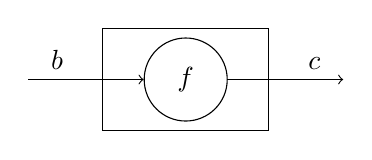
\begin{tikzpicture}[node distance=2cm]
\node[pure function] (pure) {$f$};
\node[signal function, fit=(pure), minimum width=6em] (arrf) {};
\coordinate[left of=arrf] (in);
\coordinate[right of=arrf] (out);
\draw [->, near start] (in) to node[auto] {$b$} (pure);
\draw [->, near end] (pure) to node[auto] {$c$} (out);
\end{tikzpicture}
\caption{arr $f$}
\end{figure*}
\begin{minted}{haskell}
class Arrow a where
    -- Any pure function is a generalised computation
    arr :: (b -> c) -> a b c
\end{minted}

\begin{figure*}[ht]
\centering
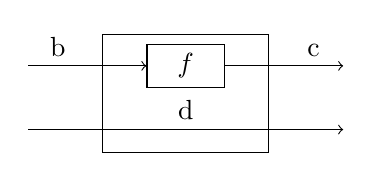
\begin{tikzpicture}[node distance=2cm]
\node[signal function, minimum width=2.8em] (f) {$f$};
\coordinate[below of=f, node distance=2.8em] (lol);
\node[signal function, fit=(f)(lol), minimum width=6em] (arrf) {};
\coordinate[left of=f] (in);
\coordinate[below of=in, node distance=2.3em] (in2);
\coordinate[right of=f] (out);
\coordinate[below of=out, node distance=2.3em] (out2);
\draw [->, near start] (in) to node[auto] {b} (f);
\draw [->, near end] (f) to node[auto] {c} (out);
\draw [->] (in2) to node[auto] {d} (out2);
\end{tikzpicture}
\caption{first $f$}
\end{figure*}
\begin{minted}{haskell}
    -- Apply the computation to part of the input, and ignore the other
    first :: a b c -> a (b,d) (c,d)
\end{minted}

\begin{figure*}[ht]
\centering
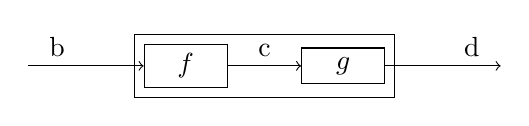
\begin{tikzpicture}[node distance=2cm]
\node[signal function, minimum width=3em] (f) {$f$};
\node[signal function, minimum width=3em, right of=f] (g) {$g$};
\node[signal function, fit=(f) (g), minimum width=6em] (arrf) {};
\coordinate[left of=f] (in);
\coordinate[right of=g] (out);
\draw [->, near start] (in) to node[auto] {b} (f);
\draw [->] (f) to node[auto] {c} (g);
\draw [->, near end] (g) to node[auto] {d} (out);
\end{tikzpicture}
\caption{$f \ggg g$}
\end{figure*}

\begin{minted}{haskell}
    -- Computations can be composed similar to (.)
    (>>>) :: a b c -> a c d -> a b d
\end{minted}

In our context, this allows us to store opaque (that is, not visible to the user) state along a function in a construct called \emph{signal functions}, which are an instance of |Arrow|.
Another instance is the pure function type \mintinline{haskell}{(->)} with rather straightforward definitions: \mintinline{haskell}{arr = id}, \mintinline{haskell}{first f = \(a, b) -> (f a, b)} and \mintinline{haskell}{f >>> g = g . f}. Every other instance has to behave more or less similar to this one due to \mintinline{haskell}{arr :: Arrow a => (b -> c) -> a b c} and internal consistency requirements mandated by |Arrow| laws\cite{Hughes98generalisingmonads}.
These are used in recent FRP frameworks such as Yampa \cite{hudak2003arrows}, Netwire \cite{haskell-wiki-netwire} and Elm \cite{elm-lang} (albeit in a less rigorous form)  and as such we'll be giving an overview over their usage.

\subsubsection{Signals and signal functions}
\begin{figure}[ht]
\centering
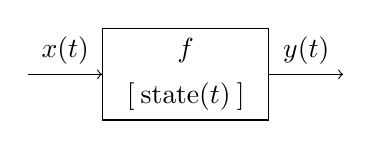
\begin{tikzpicture}[node distance=2cm]
\node[signal function with state, minimum width=6em] (arrf) {$f$ \nodepart{second} $[\: \operatorname{state}(t) \: ]$};
\coordinate[left of=arrf] (in);
\coordinate[right of=arrf] (out);
\draw [->] (in) to node[auto] {$x(t)$} (arrf);
\draw [->] (arrf) to node[auto] {$y(t)$} (out);
\end{tikzpicture}
\captionof{figure}{Signal function}
\label{fig:sigfunc}
\end{figure}

A \emph{signal} is essentially a |Behaviour| from classical FRP --- a value changing over time.
\emph{Signal functions} are, as the name suggests, functions on signals, but also encapsulate state that is only dependent on the input history. State isn't always used; for instance |integral| is a stateful function while |arr| is stateless. That is, the output \(y(t)\) of a stateless function \(f(x)\) is only dependent on the input \(x(t)\), whereas for a stateful function $f(x, state)$ the output depends on a state function \(\operatorname{state}(t)\). This state function summarises the input history \(x(t')\) over the interval \(t' \in [0,t]\). It is also useful that signal functions can inhibit --- that is, produce no value at all, similar to how \mintinline{haskell}{data Either a b = Left a | Right b} is used for error catching with \mintinline{haskell}{Left} and the actual value with \mintinline{haskell}{Right}. Using that you can still have a total signal function while supporting missing values --- if you were to use |undefined| or a similar bottom value, your program would either crash or not perform properly\footnote{due to the denotational semantics of bottom values, meaningful pattern matching on them is fundamentally impossible; trying to do e.g. \mintinline{haskell}{case head xs of undefined -> 1; 'a' -> 0} would give a warning about overlapping pattern matching and always evaluate to 1, regardless whether |xs = []| or |xs = "a"| or anything else)}.

For the purpose of game programming, we'll present a few combinators that are especially important. For the sake of simplicity, we'll define |SF a b| as a concrete signal function mapping a to b. Furthermore, we'll use monomorphic types like |Float -> Int| even when the underlying concept is valid for constrained polymorphic types like |Fractional a, Integral b => a -> b|. It should be noted that this is list is far from exhaustive and is only intended as an overview.

\begin{itemize}
\item In most games, movement input is mapped to change in velocity. In order to convert a velocity signal into a position signal, you need to integrate it: $x(t) = \int_{t_0}^t v(t') dt'$. This is pretty similar to a stateful signal function, and indeed it is. 
\begin{figure}[ht]
\centering
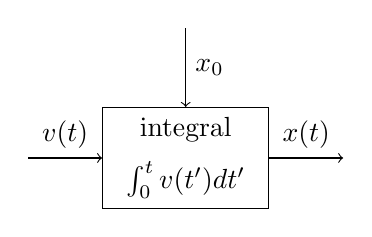
\begin{tikzpicture}[node distance=2cm]
\node[signal function with state, minimum width=6em] (integral) {integral \nodepart{second} $\int_0^t v(t') dt'$};
\coordinate[left of=integral] (in);
\coordinate[right of=integral] (out);
\coordinate[above=1cm of integral] (opt);
\draw [->] (in) to node[auto] {$v(t)$} (integral);
\draw [->] (integral) to node[auto] {$x(t)$} (out);
\draw [->] (opt) to node[auto] {$x_0$} (integral);
\end{tikzpicture}
\end{figure}
For example, you could write \mintinline{haskell}{speed >>> integral 0} to construct a position signal function, and \mintinline[breaklines]{haskell}{gravity >>> integral 0 >>> integral 100} to do the same for a object in free fall from 100m.

\item A set of signal functions operating on intervals. For example, \mintinline{haskell}{after :: Time -> SF a b} produces a value after a time period, \mintinline{haskell}{for :: Time -> SF a b} produces a value for a time period, and so on. \mintinline{haskell}{after 60 >>> for 70 >>> gameOver} would give you a 60 second time limit on your game, after which a game over screen displays for ten seconds (after that the wire inhibits forever). Note that \mintinline{haskell}{(>>>)} does not reset local time (unlike switching, detailed below) and as a result \mintinline{haskell}{after}, \mintinline{haskell}{for} and \mintinline{haskell}{gameOver} are at the same time at all times, even if they're not actually being evaluated. This leads to $70 - 60 = 10$ seconds of game over screen being shown.

\item In order to respond to discrete occurrences, we use an |Event| type similar to classical FRP. Let's say we want to start moving left when the |A| key is held down. The signal function \mintinline{haskell}{between :: SF (a, Event b, Event c) a} inhibits until the left event occurs and then produces until the right event happens. If we define \mintinline{plain}{keyUp, keyDown :: SF Key (Event Key)} we can then write (using Arrow do-notation\cite{ghcdocs-arrownotation}, which for the intents of this paper can be read just like regular, monadic do notation with |proc x| replaced by |\x|)
\begin{minted}{haskell}
moving Left = proc x -> do
    down <- keyDown "A"
    up <- keyUp "A"
    between (x, down, up)
\end{minted}
\begin{figure}[ht]
\centering
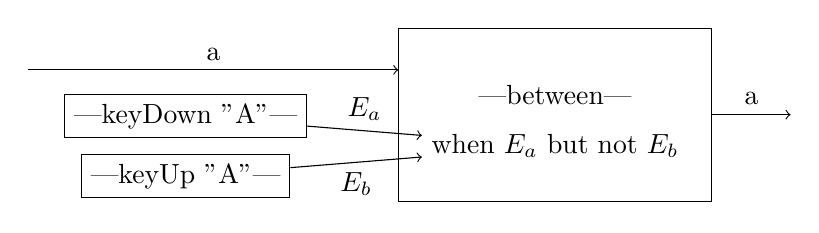
\begin{tikzpicture}[node distance=2cm]
\node[signal function, minimum width=7em] (kd) {|keyDown "A"|};
\node[signal function, minimum width=7em, below=0.2cm of kd] (ku) {|keyUp "A"|};
\coordinate (key) at ($(kd)!0.5!(ku)$);
\coordinate[above=1.25cm of key] (a);
\coordinate[right=3cm of a] (b);
\node[auto, right=3cm of key] (cond) {when $E_a$ but not $E_b$};
\coordinate[below=0.5em of cond] (align);
\coordinate[left=0.5em of cond] (coll);
\coordinate[right=0.5em of cond] (sym);
\node[signal function with state, fit={(b) (cond) (coll) (sym) (align)}] (between) {|between| \nodepart{second}};
\draw[->] (kd) to node[above] {$E_a$} (cond);
\draw[->] (ku) to node[below] {$E_b$} (cond);

\coordinate (reala) at ($(a) + (-2cm,-8pt)$);
\draw [->] (reala) to node[above, midway] {a} (reala-|between.west);

\coordinate[right=1cm of between] (out);
\draw [->] (between) to node[above] {a} (out);
\end{tikzpicture}
\end{figure}
In fact, this is just syntactic sugar for \mintinline{haskell}{arr}, \mintinline{haskell}{first} and \mintinline{haskell}{(>>>)}, but the resulting expression would be much more complicated to understand, which is why we chose to use do-notation here.

\item All of our previously introduced signal functions can only evolve with time, not be replaced with some other combinator when something happens. For this we use \emph{switching}, with the most important operator being \mintinline{haskell}{(-->) :: SF a b -> SF a b -> SF a b}.
When you have \mintinline{haskell}{f = f1 --> f2}, then \mintinline{haskell}{f = f1} as long as f1 doesn't inhibit. When it inhibits, the signal function permanently switches to \mintinline{haskell}{f = f2}.

As an example let's implement elastic collision with a surface.
\inputminted[breaklines=true]{haskell}{Switch.hs}
The |when| combinator inhibits when the predicate evaluates to |False|, so until we reach the wall's position we move. Once that happens we switch and start moving backwards.

Note that when a switch occurs, local time resets. For example, \mintinline[breaklines]{haskell}{f = pure 1 >>> for 3 --> pure 2 >>> at 3} would evaluate to 1 from $t=0$ to $3$, inhibit for $t=3$ to $6$ and then produce $2$ forever after $t=6$ since as soon as \mintinline{haskell}{for} inhibited, the switch occured to \mintinline{haskell}{at}, which then starts producing after 3 seconds. Similarly, \mintinline{haskell}{g = pure 1 >>> for 1 --> pure 0 >>> for 1 --> g} would create a periodical signal function oscillating between 1 and 0 each second.
\end{itemize}

\section{FRP frameworks}
\label{sec:frameworks}
\subsection{Elm}
Elm is a basic functional programming language which comes with many features.
One of those features is the Time Traveling Debugger\cite{elm-debugger} which allows the developer of a game to see the change of it over the time and lets him travel forward and backward in his program to seek out bugs.
It allows us to track our data and visualise our program.
We could track our main character. Then we would analyse their respective record\cite{elm-record}. A data structure which we use to store data related to our character similar to objects..
Then we could see our bugs unwind and analyse what causes them so we are able to fix them easily.
Another benefit is the feature of hot-swapping\cite{elm-swapping} which allows us to program more interactively as we modify running code.
Hot-swapping is made possible in Elm through the separation of state and function which is achieved through purity.
This means that we will always get the same results for the same arguments.
Combined with the immutability of data we will get the same results when we rewind our Program without destroying our data.
This is hardly achievable in imperative languages as they feature destructive updates.
Those features are combined in the Elm Reactor\cite{elm-reactor} which is a development tool providing us with a strong foundation to maintain our program.
At the core of an implementation of FRP with Elm is the use of Signals\cite{elm-signal}
Elm provides us with a network that processes those signals for us called a signal graph.
This makes the use of signals and programming functionally reactive easy.
Another important basis for the implementation of our game is to provide a state for our game.
Elm allows us to inhibit signals by the use of the foldp\cite{elm-signal} function.
This function takes an update function, our starting state, and a signal as input returning a Signal.
foldp does this by applying our update function every time our signal occurs onto our starting state returning a Signal representing our current state.
\newline
\begin{minted}{haskell}
foldp : (a -> state -> state) -> state -> Signal a -> Signal state
\end{minted}
Additionally through the use of an update function we can store data with this function such as mouse clicks.
{\tt mouseClicks} tracks the count of incoming mouse clicks.
\newline
\begin{minted}{haskell}
clickCount = foldp (\click count -> count + 1) 0 Mouse.clicks
\end{minted}
Here our {\tt mouse.clicks} signal triggers our update function which increments our counter starting at 0 every time a mouse click occurs.
Now we are provided with our functional implementations of state, objects and input giving us the basis to create games.
\section{A functional game}
\label{sec:game}
In the following section we are going to implement pong with Elm according to the paradigms of FRP.
But first we have to understand the basic structure of most games including pong in Elm.
\subsection{Elm's architecture}
In imperative language you can reach into objects and data structure at any given time.
With functional programming languages we do not have this luxury as a programmer.
Therefor we need to structure our code accordingly so we have the data at hand when we need it.
A common architecture for this is the Model-View-Controller architecture\cite{wiki-mvc} that is used widely in multiple domains of programming such as web applications to structure code. 
Elm's common architecture\cite{elm-mvc} resembles this closely but isn't exactly the same.
Elm's architecture divides our code into 4 parts.
First one being the input in which we take our input from outside in our example the keyboard and the time which is given to us through signals.
This part is often called the signal section as well as we string together our input streams in this section.
The update takes our input and defines functions to move our game forward by changing the information of our model or how our view is being displayed.
This is described as the controller in a classic MVC-architecture but in Elm this is split into 2 parts.
The model stores most of the data of our game which is needed for our view, update and input to work.
The view implements our visual representation of our game.
It requests the information of our model according to our update every time an input occurs to represent our game.
By separating our code into those parts we can change each easily without messing with our code.
\subsection{Our Game}
The first part of our game is importing the required libraries for our game.
We import graphics, color and text libraries so we can easily display our pong court with written instructions on it.
We need the keyboard and time libraries for our input.
Lastly we need a window library to render our game. 
\inputminted [breaklines=true] {haskell}{pong(1).hs}
\subsection{Model}
First off we define our Pong Court with
\inputminted [breaklines=true] {haskell}{pong(2a).hs}
This makes it easier to change our court later on in the game development.
Next we define a Union Type which behaves like our user-defined types in Haskell.
This allows us to enumerate possible states.
In this cast {\tt State} is used to store if our game is running in play our being paused and has yet to start.
\inputminted [breaklines=true] {haskell}{pong(2b).hs}
Now we define multiple type aliases. Those are used to have an alias declaration for our declared type in this case our records\cite{elm-record}.
A record is a data type which stores multiple values of different types similar to structures in C.
Type aliases and records combined allow us to define our own data types with a custom name as a synonym for said type making our game more concise and easier to understand.
Our first one being the ball. 
Here we need a type alias representing a record which stores the position and velocity of the ball.
We break this data down into their x and y components.
\inputminted [breaklines=true] {haskell}{pong(3a).hs}
Second we define the same properties for our {\tt Player} type alias which represent the paddle and its according position and movement but each player can score so we store their score as well.
\inputminted [breaklines=true] {haskell}{pong(3b).hs}
The next type alias represents all our game items. Our 2 players, the game state and our ball.
\inputminted [breaklines=true] {haskell}{pong(3c).hs}
Lastly we have a type alias for the input.
We store a Boolean called space to check if the space bar was pressed and we can therefor start the next round.
We store 2 directions with an integer. 
This integer is 1 if our players press w or cursor up to move their respective paddle upwards. 
It is 0 the players are not pressing up or down. 
It is -1 if they press s or cursor down to move their respective paddle downwards.
\inputminted [breaklines=true] {haskell}{pong(3d).hs}
Now we introduce 2 functions to initialise our type aliases in their default position.
{\tt player} takes in a float and returns a {\tt Player} type with all values besides our x-coordinate set as 0.
Our x-coordinate is set with the value of our input floating-point number.
\inputminted [breaklines=true] {haskell}{pong(4a).hs}
The {\tt defaultGame} uses this function to initialise the default game.
It starts with the state being {\tt Pause} and the ball at {\tt (0, 0)} with a velocity of 200 units on each axis.
The players are set according to the player function on opposing sides of the court.
\inputminted [breaklines=true] {haskell}{pong(4b).hs}
\subsection{Input}
To track the time our game implements a time delta which is defined by the {\tt fps}\cite{elm-time} function.
{\tt fps} takes in a number of frames per second and the resulting signal returns a sequence of time deltas.
This sequence to correlates to the input amount of frames.
With {\tt inSeconds} we take the Elm's underlying units of time and transform them into their respective values expressed in seconds. 
\inputminted [breaklines=true] {haskell}{pong(5a).hs}
Now with our time set we can define our current input every time our time delta occurs.
That is achieved by the {\tt sampleOn}\cite{elm-sampleOn} function that takes a sample from our second input signal (Our keyboard and time input) every time our first input signal occurs returning us a signal of samples.
Here we model our paddles direction through the use of the keyboard library.
Whenever a signal occurs through pressing wasd-keys or arrow-keys our WASD and arrows function return an record storing an integer for the x and y directions.
With the appliance of {\tt .y} onto those functions we only receive the y component.
Through the definition of {\tt WASD} and {\tt arrows} we receive 1 for an upwards direction through the use of w or the up arrow and -1 with s and the down arrow.
0 is returned if no button or those with no impact on our y component were pressed.
Note the use of {\tt\textless$\vert$}.
{\tt\textless$\vert$} and {\tt$\vert$\textgreater} are operators to apply functions to avoid parentheses.
In our case {\tt\textless$\vert$} takes the input on the right and applies it as a parameter of {\tt sampleOn}.
\inputminted [breaklines=true] {haskell}{pong(5b).hs}
\subsection{Update}
To progress our game forward we will implement the update section of our game.
First we break our interactions into smaller function to structure our code.
{\tt near} checks if {\tt k} is within {\tt c} of {\tt n} which will be used to check for collisions of our ball and the player's paddles.
\inputminted [ breaklines=true] {haskell}{pong(6).hs}
{\tt within} uses near to check if the ball is within the paddles collision box. .
We check if the ball is within 8 units of our x-axis to the players paddle and 20 units within the y-axis to validate if the ball is near a paddle.
\inputminted [breaklines=true] {haskell}{pong(7).hs}
{\tt stepV} changes our velocity according to a collision.
According to the type of the collision the direction of our ball is changed with {\tt abs v} which turn our negative velocity value into a positive or vice versa with {\tt 0 - abs v}.
If no collision is occurring the ball keeps moving without alternation.
We will iterate this to update the position and velocity of our ball.
\inputminted [breaklines=true] {haskell}{pong(8).hs}
Next is {\tt physicsUpdate} that is used to translate the values of velocity of our players and the ball to their new position with each occurrence of our time delta.
This allows us to actually display movement.
Here we update our variable according to Elm's syntax as we access our record left of {\tt$\vert$} and update our variables left of {\tt \textless-} to their new values on the right.
We can update as many fields of our record as we like separating each update by a comma.
Note here that Elm supports structural typing\cite{wiki-structural-type} to give {\tt physicsUpdate} a record with {\tt {x, y, vx, vy}} as structural elements as an input object.
This way we can use the player and the ball record as a input for this function. 
\inputminted [breaklines=true] {haskell}{pong(9).hs}
Now onto our major functions which step our basic elements of our game forward.
We start with analysing our {\tt updateBall} function.
Here we progress the position of {\tt Ball} according to time and his positional relation to each players paddle.
We first check if the ball is out of bounds through checking if the ball is near a {\tt halfWidth} of our court to 0.
This is not the case when a player has scored moving the ball behind the enemy's paddle outside the court.
If this occurs we set the ball to {\tt (0, 0)}.
\inputminted [breaklines=true] {haskell}{pong(10a).hs}
if the ball is within the court we update the position of our ball with {\tt physicsUpdate}.
We update {\tt vx} and {\tt vy} through the use of {\tt stepV} to check for any occurring collisions.
Those collisions could occur at the players paddle or on the horizontal limits of our court.
\inputminted [breaklines=true] {haskell}{pong(10b).hs}
{\tt updatePlayer} is implemented to update our player's paddles and scores according to their keyboard input and scored points.
Here we use Elm's let expressions that first defines values with let and with in we apply those values. 
The first part of this structure is called the let-expression while the second part where we apply our predefined values is called the where-expression.
First we define {\tt player1} which is defined through our input {\tt player}.
His paddle position is updated according to the current input through the appliance of {\tt physicsUpdate}.
{\tt physicsUpdate} applies an updated {\tt vy} representing the player's current input.
\inputminted [breaklines=true] {haskell}{pong(11a).hs}
Next we use  that definition to keep our player's paddle in court with the use of {\tt clamp}\cite{elm-basics}.
{\tt clamp} takes 3 numbers as an input and returns a number.
{\tt clamp} checks if the the last input number is with the span of the first two and returning the number in that case.
If our last input number exceeds our lower or upper bound it returns the exceeded bound.
This way we can use {\tt clamp} to restricts our values for {\tt player1.y} to our first two inputs thus keeping our paddles within the court.
Additionally we update our players score by adding our input points onto the players already existing ones.
\inputminted [breaklines=true] {haskell}{pong(11b).hs}
Now we combine all those integral parts into on big update function that updates our whole game.
It takes our input and our current game state which includes our state, our ball as well as our 2 players returning us with an updated, current game state.
In our let-expression we define two scores to store which player scored this round.
We implement this by checking on which side of the court the ball went out of bounds.
This can be evaluated through comparing our balls position on the x-axis compared to half the width of our court.
\inputminted [breaklines=true] {haskell}{pong(12a).hs}
Following we define the {\tt newState}.
If space was pressed we set our state to {\tt Play}. 
If the {\tt score1} is not the same as {\tt score2} which occurs when a player has scored we pause our game for the next round.
If nothing occurs our state remains.
\inputminted [breaklines=true] {haskell}{pong(12b).hs}
Next we define our {\tt newBall} which remains as it is if the game is paused.
Otherwise it gets updated according to {\tt updateBall} if the game is running.
\inputminted [breaklines=true] {haskell}{pong(12c).hs}
In our where expression the game is updated accordingly to our previously updated elements of our game.
\inputminted [breaklines=true] {haskell}{pong(12d).hs}
\subsection{View}
Now that all is set we have to implement our view so we can render the game.
As we did in our update section we first define a few helpers to structure our code.
First we define 2 colours for our pong court and text as well our on screen message itself.
\inputminted [breaklines=true] {haskell}{pong(13a).hs}
Our next function uses a very interesting concept of compositions.
{\tt\textgreater\textgreater} passes along the results of our first function to the next one.
Trough the use of {\tt\textgreater\textgreater} and {\tt\textless\textless} we can compose functions with one another and run them successively.
In this case we transform our string {\tt f} to Elm's type {\tt Text} so we can use Elm's {\tt color} function and and use monospace as a font lastly our text will be made left aligned.
\inputminted [breaklines=true] {haskell}{pong(13b).hs}
{\tt make} is used to create elements for our objects such as the paddles, the field and the ball.
It creates an element according to the input shape and moves it to the location stored in the the object.
\inputminted [breaklines=true] {haskell}{pong(13c).hs}
{\tt view} takes a integer tuple and our current game state to represent it visually as an {\tt Element}.
With our let expression we define scores returning an {\tt Element} to display our current scores onto the court.
We use our {\tt txt} function in this expression to transform our input text into an {\tt Element}.
\inputminted [breaklines=true] {haskell}{pong(14a).hs}
In our where expression we implement elements for our pong court, our ball, our 2 paddles for our respective players as well as a score counter and our on screen information that is only displayed when the game is paused.
\inputminted [breaklines=true] {haskell}{pong(14b).hs}
\subsection{Combining the pieces}
This is usually a part of the input section but has been moved towards the end for the sake of a more comprehensible structure of explanation.
{\tt gameState} is implemented to store our game state through the use of {\tt foldp}.
We apply our update function onto our {\tt defaultGame} every time an input occurs.
\inputminted [breaklines=true] {haskell}{pong(15).hs}
Now finally we finished all of our game and put it together in one tiny main function.
{\tt map2} here is used to apply a function onto 2 signals return one signal.
So we apply {\tt view} every time our {\tt gameState} our our window dimensions change and are able to run our game.
\inputminted [breaklines=true] {haskell}{pong(16).hs}
\subsection{Summary}
To create our game we first implemented data structures to model our objects through the use of union types and type aliases as well as a function to define their default game state.
Then we implemented the passage of time and following our input as it relies on our delta to function.
As we lay the ground for our game we implemented our update section that we build first from basic interactions to check positional differences, collisions and to apply velocity.
This was then combined into larger functions to update our ball's and our player's state which was further combined into one big update function which updates the whole game's state.
Now we provided visuals with our view section through the use of our graphical libraries through creating different shapes and texts.
Lastly we implemented our {\tt gameState} function that updates our {\tt defaultGame} according to our input with the update function.
With all this implemented we could set up our main function that represents the view according to the game's state and the window's dimensions.

\section{Related works}
\label{sec:related}
Conal Elliott's paper "Push-pull functional reactive programming" \cite{Elliott2009-push-pull-frp} serves an integral role in modern FRP
and serves as the theoretical basis of many FRP libraries. Alexander Berntsen master thesis on programming game systems in Haskell \cite{Berntsen2014-game-systems-haskell} compares imperative and functional game design based on a medium-sized game and provides substantial evidence supporting the usage of strongly static typed purely functional programming for game development. Charles' post about recreating Asteroids in Netwire \cite{asteroids} describes difficulties encountered when implementing a game using Netwire.
Evan Czaplicki's implementation and blog about making pong\cite{elm-pong, elm-making-pong} serves as the exemplary game to showcase in Elm.
\section{Conclusion and Outlook}
\label{sec:conclusion}
Game programming using FRP allows for faster and cleaner development, but it's also not a panacea --- without additional care (such as push-pull FRP\cite{Elliott2009-push-pull-frp} and various optimisations) performance and space leaks become an issue. Additionally, the paradigm shift from imperative to purely functional reactive programming is quite extreme, requiring a comparatively large training period. The amount of actively developed FRP game engines is fairly low\cite{hackage-frp}, so solutions using Haskell might need a custom game engine. However with increased usage of FRP for game development this should become less of an issue.

The actual implementation of FRP is beyond the scope of this paper, and implementers of game engines or similar should consult references and their framework's internal documentation.

\bibliographystyle{plain}
\bibliography{references}
\end{document}